\documentclass{article} % For LaTeX2e
\usepackage{nips14submit_e,times}
\usepackage{hyperref}
\usepackage{url}
\usepackage{graphicx}
\usepackage[super]{nth}
\usepackage{todonotes}
\usepackage{amsfonts}

%\documentstyle[nips14submit_09,times,art10]{article} % For LaTeX 2.09

\title{CPSC 536N Project: Gossip Protocols with Random Linear Network Coding}
\author{
Neil~Newman\\
81435142\\
Department of Computer Science\\
University of British Columbia\\
Vancouver, BC V6T 1Z4 \\
\texttt{newmanne@cs.ubc.ca}
}
\newcommand{\fix}{\marginpar{FIX}}
\newcommand{\new}{\marginpar{NEW}}

\def\numNodes{\textit{n}\,}
\def\graph{\textit{G(t)}\,}
\def\graphtime{\textit{t}\,}
\def\numMessages{\textit{k}\,}
\def\RLNC{\textit{RLNC}\,}
\def\fieldSize{\textit{q}\,}

\nipsfinalcopy % Uncomment for camera-ready version

\begin{document}

\maketitle

\section{Introduction}
\paragraph{Gossip Protocols}
Gossip protocols are randomized algorithms used to spread information, namely a set of messages, within a network. Gossip protocols are modeled on the way that rumours spread among a society or the way in which a disease outbreak spreads throughout a population (gossip protocols are sometimes referred to as epidemic protocols). Initially, information is spread throughout the network (each node may know none, part, or all of the information), and the goal is to make every node in the network know all of the information. The protocol achieves this through a series of pairwise interactions between nodes in which knowledge is exchanged. In contrast to non-randomized algorithms, gossip algorithms do not take the structure of the network into account. This fact makes gossip protocols suitable for use in real networks, in which communication links can fail and network topologies can evolve over time. In contrast, a non-randomized approach, such a constructing a spanning tree, would require a known and stable network. 

\paragraph{Random Linear Network Coding}
One issue with gossip protocols is that if the goal is to spread multiple messages in parallel, a node need to choose which information it sends in each interaction without knowledge of what the other node knows or does not know (acquiring this knowledge would be expensive, as would be sending all of the information that it knows). If the node were to simply choose a random message that it knew about, it is possible for some messages to become widely spread while others remain rare, so that the stopping time for the algorithm, (the point at which every node knows all of the messages) could be dominated by the time it takes to propogate the rare messages. This can be circumvented by using gossip protocol based on \emph{Random Linear Network Coding} (RLNC). In this protocol, discussed in more detail in \ref{subsec:RLNC}, a node sends a message that is a random linear combination of the messages that it knows. The original messages can be recovered using Gaussian elimination once a node has received enough linearly independent coefficient vectors--however, it should be noted that until this time, it is possible that the node will not be able to decode any of the individual messages (i.e. it can be all or nothing).

\paragraph{Rumor Mongering}
Rumor mongering is another method of distributing information. When a node receives a message, the message is a \textit{hot rumor}. As long as the rumor is hot, the node will periodically connect with another random node and see if it knows about the rumor. If the node tries to share a rumor and the other node already knows about it, then the rumor cools off. Eventually, the node stops propagating the rumor entirely. 

\paragraph{Anti-entropy}
A node chooses another node at random and performs a complete exchange of knowledge. This is prohibitively expensive, but can be used occasionally to guarantee eventual consistency.

\paragraph{Applications}
Gossip protocols can be applied to database replication as demonstrated in \cite{demers1987epidemic}. 

\subsection{Model of Network and Communication}
We will use the model from \cite{haeupler2011analyzing}, which is as follows: There are \numNodes nodes in the network. A network is a graph \graph that can be static ($\graph = G  \forall \graphtime$) or can vary with time \graphtime and is either directed or undirected. An edge in \graph from any two nodes \textit{a} and \textit{b} represents a link through which communication can take place in round \graphtime; if the edge is directed it means that communication can only occur in the direction of the edge. We will assume that \graph is connected at every \graphtime, however this requirement can be weakened. 

\subsection{Message structure}
There are \numMessages distributed over the network (see \ref{subsec:startingconditions} for details on the ways in which we consider the messages to be distributed). 

\subsection{Additional assumptions}
Packets are never dropped. All packets have the same size. 

\subsection{Modes of communication}
We allow the following four modes of communication:
\begin{itemize}
\item \texttt{BROADCAST} A node sends to all of its neighbours
\item \texttt{PUSH} A node sends to one neighbour chosen uniformly at random
\item \texttt{PULL} A node chooses a neighbour uniformly at random and receives a message from the neighbour
\item \texttt{EXCHANGE} A node chooses a neighbour uniformly at random and they each send each send each other a message
\end{itemize}
The choice of what packet to send is never conditioned on the who will receive the packet.

\subsection{Timing models}
We consider synchronous models in which every node in the network can send a message once per round. Asynchronous models have also been studied in the literature.

\subsection{Starting conditions}\label{subsec:startingconditions}
We consider the following starting conditions:
\begin{itemize}
\item \texttt{DISTRIBUTED} Each node knows a single, unique message
\item \texttt{SINGLE} A single node knows every message, other nodes know nothing
\end{itemize}

\subsection{Graph types}
\begin{itemize}
\item \texttt{COMPLETE} Every node is connected to every other node
\item \texttt{ADVERSARIAL} An adversary gets to choose the set of edges at every time \graphtime (subject to the constraint that \graph must remain connected). For example, if there is only a single message to distribute, an adversary might choose to only put a single link between the set of nodes that know the message and the set of nodes that don't know the message. 
\end{itemize}

\subsection{RLNC Algorithm}\label{subsec:RLNC}
\paragraph{Preliminaries}
Packets are vectors over a finite field $\mathbb{F}_{\fieldSize}$, where the size of the field, \fieldSize, is a prime or prime power. There are \numMessages messages, $\vec{m_{1}}...\vec{m_{\numMessages}}$ that are vectors from $\mathbb{F}_{\fieldSize}^{l}$. Packets are of the form ($\vec{\mu}, \vec{m}$), where $\vec{m} = \sum_{i=1}^{\numMessages} \mu_i\vec{m_i} \in \mathbb{F}_{\fieldSize}^{l}$ and $\vec{\mu} = (\mu_1,...,\mu_k) \in \mathbb{F}_{\fieldSize}^{\numMessages}$ is the coefficient vector. Note that if a node ever knows enough coefficient vectors such that the span of these vectors equals $\mathbb{F}_{\fieldSize}^{\numMessages}$ then Gaussian elimination can be used to reconstruct all of the messages. Therefore, a minimum of \numMessages packets with linearly independent coefficients are needed. The choice of \fieldSize is a trade-off between the size of messages in bytes and the convergence rate. 
\paragraph{Algorithm}
Every node \textit{v} keeps a subspace $X_v$ that is the span of all of the coefficient vectors it currently knows. When a packet needs to be chosen to send, a node chooses a packet uniformly at random from $X_v$. When a packet is received, $X_v$ is recomputed. If $X_v = \mathbb{F}_{\fieldSize}^{\numMessages}$ then a node can decode messages. When this is true for every node, the algorithm is considered to have stopped. 
\paragraph{Practical Details}
Every node maintains only messages that are \textit{helpful}, that is, messages that increase the dimensionality of $Y_v$. Each node maintains a matrix of helpful coefficients. To determine whether or not a new message contains helpful coefficients, we compute the rank of the current matrix and the rank of the current matrix with an additional row for the message's coefficients. If the rank has increased, the message is helpful and we add it to the node's collection. Otherwise, the message is ignored. When the rank of the coefficient matrix is equal to the number of messages, a node can decode all of the messages. When this condition is true for every node, we say that the algorithm has terminated.

\subsection{Summary of theoretical results}
\paragraph{Complete graphs}
On a complete graph, RLNC gossip achieves $O(\numMessages + T)$, where $T$ is the time that it takes to distribute a single message amongst all of the nodes. This is referred to as \textit{perfect pipelining}. In a complete graph, $T$ is $O(\log{n})$. 

\subsection{Practical details}
Experiments were performed using \textit{python} and \textit{sage}. The \textit{networkx} library was used to generate graphs.

\subsection{Results}
\begin{figure}
\centering
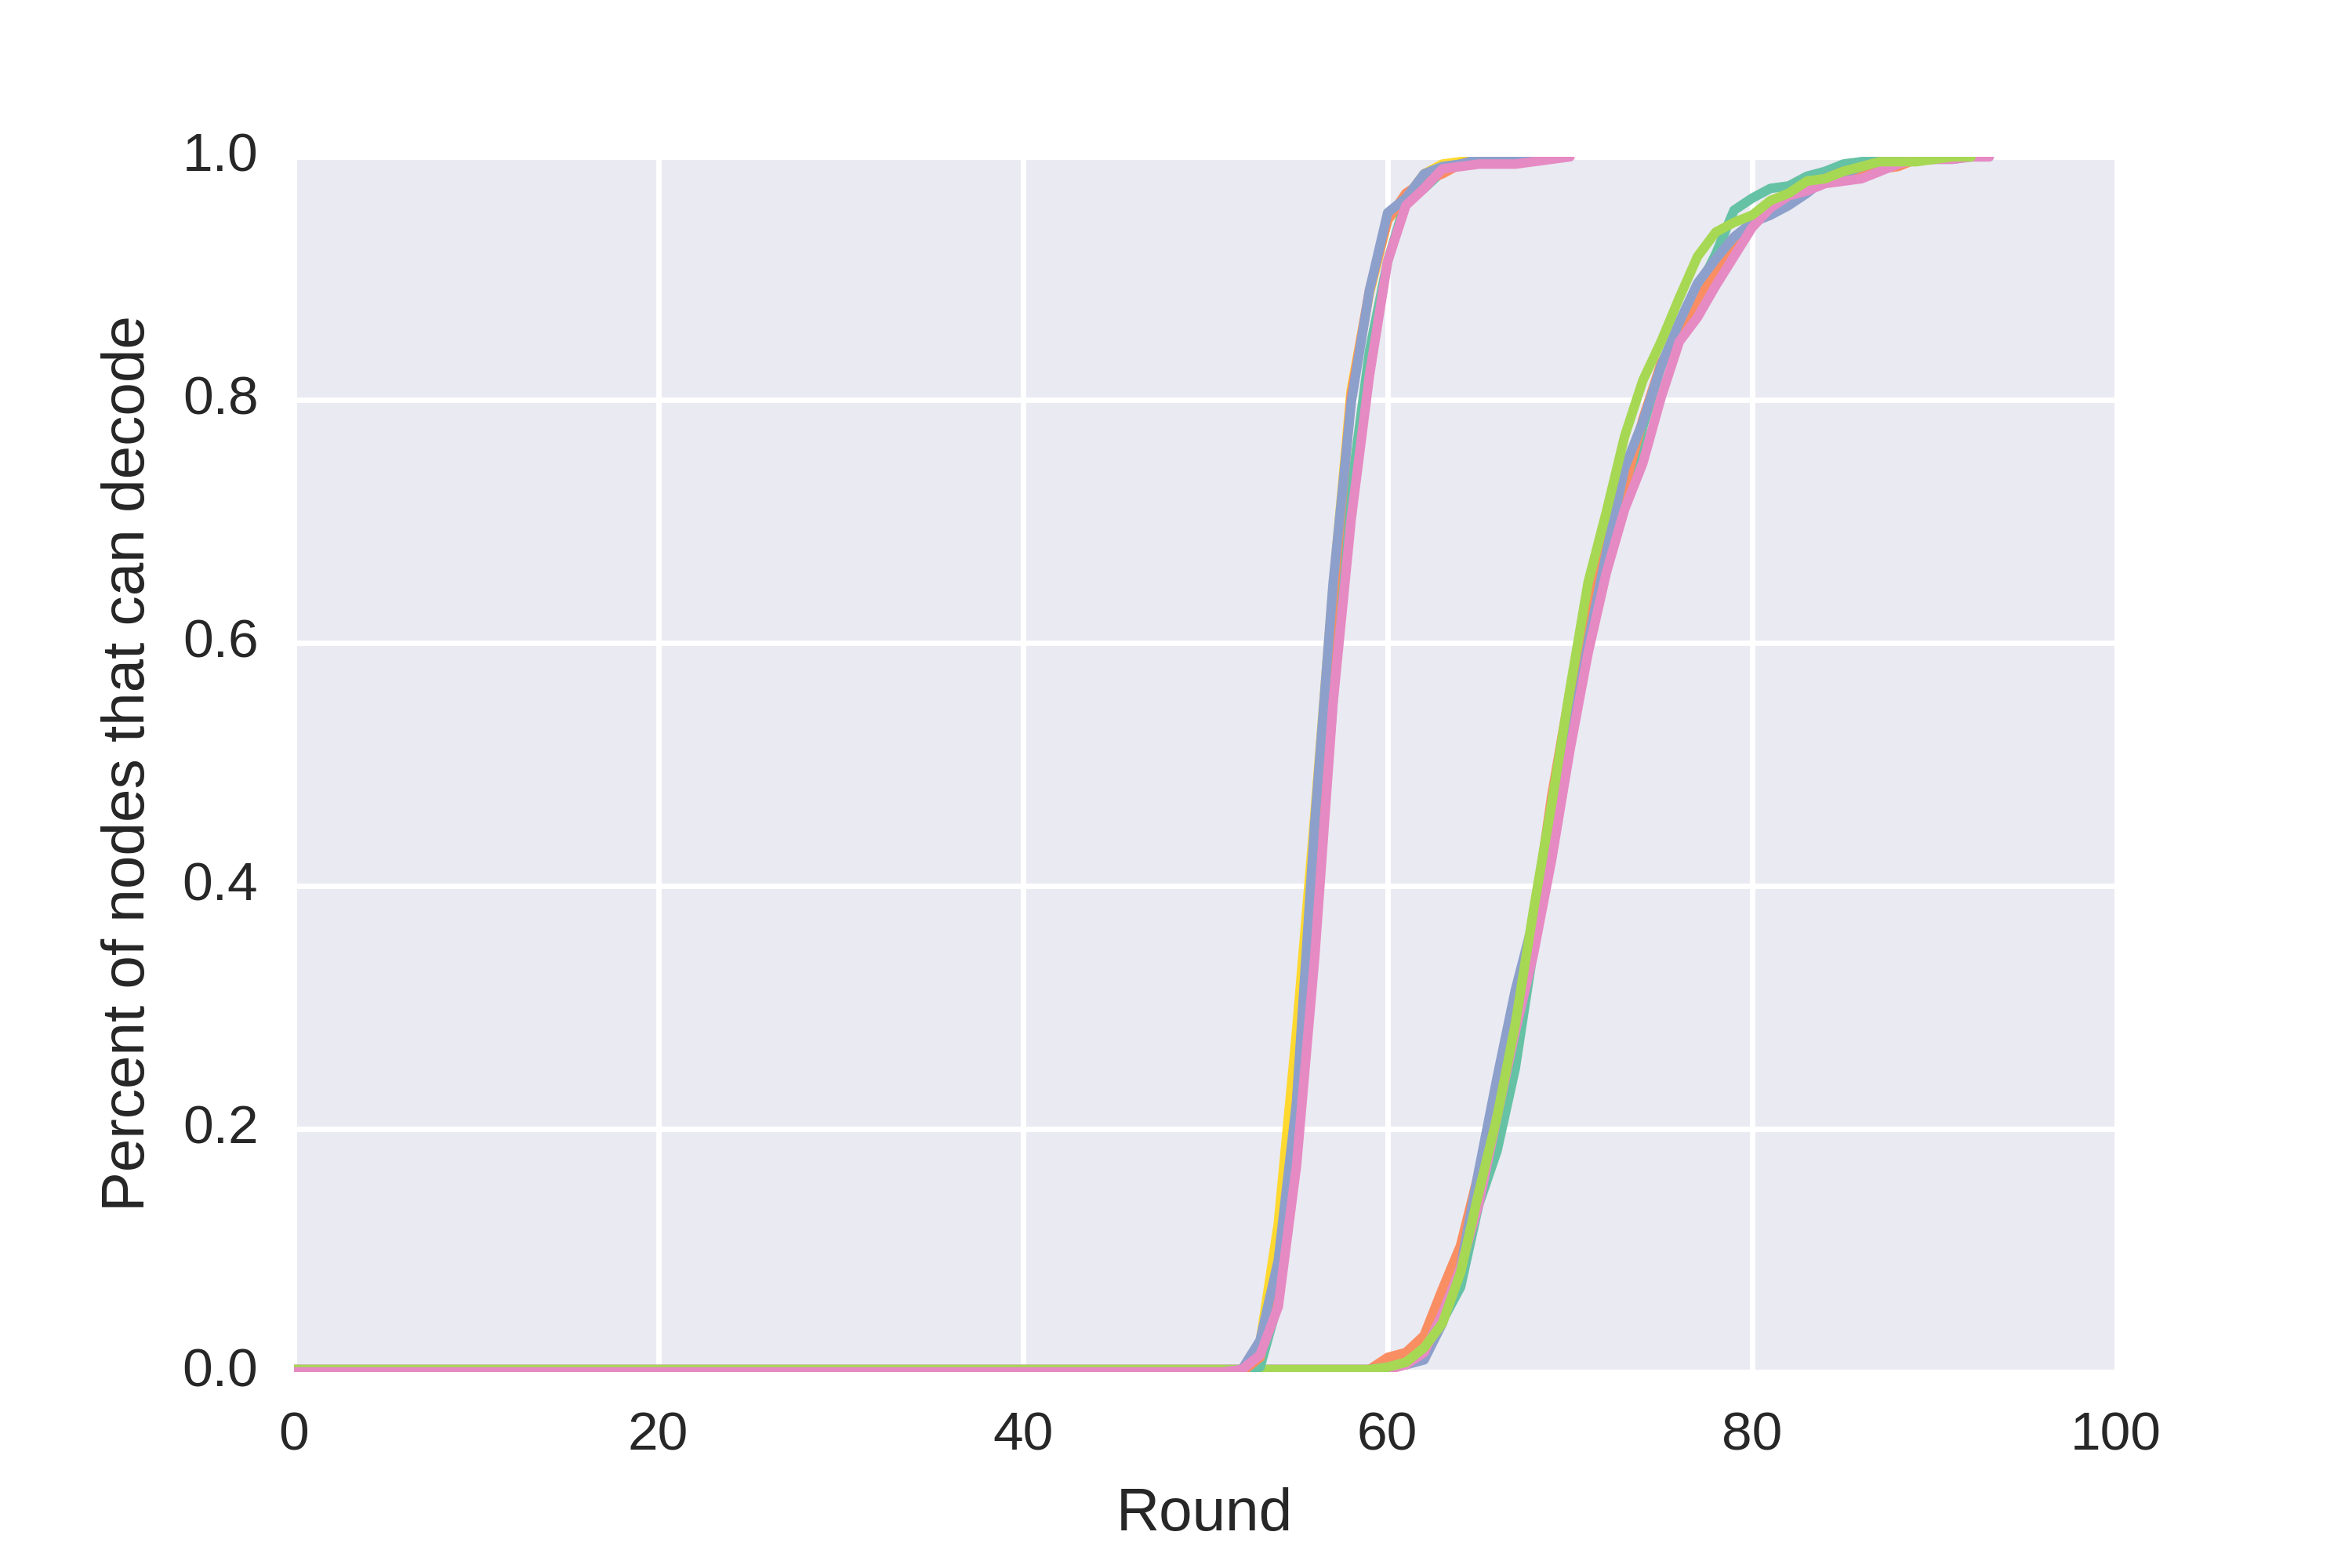
\includegraphics[width=\linewidth]{figures/rlnc-ecdf.png}
\caption{Cumulative distribution showing what fraction of nodes can decode the messages at any given round. 5 trials were performed using 500 nodes and 50 messages.}
\label{fig:rlnc-ecdf}
\end{figure} 
\begin{figure}
\centering
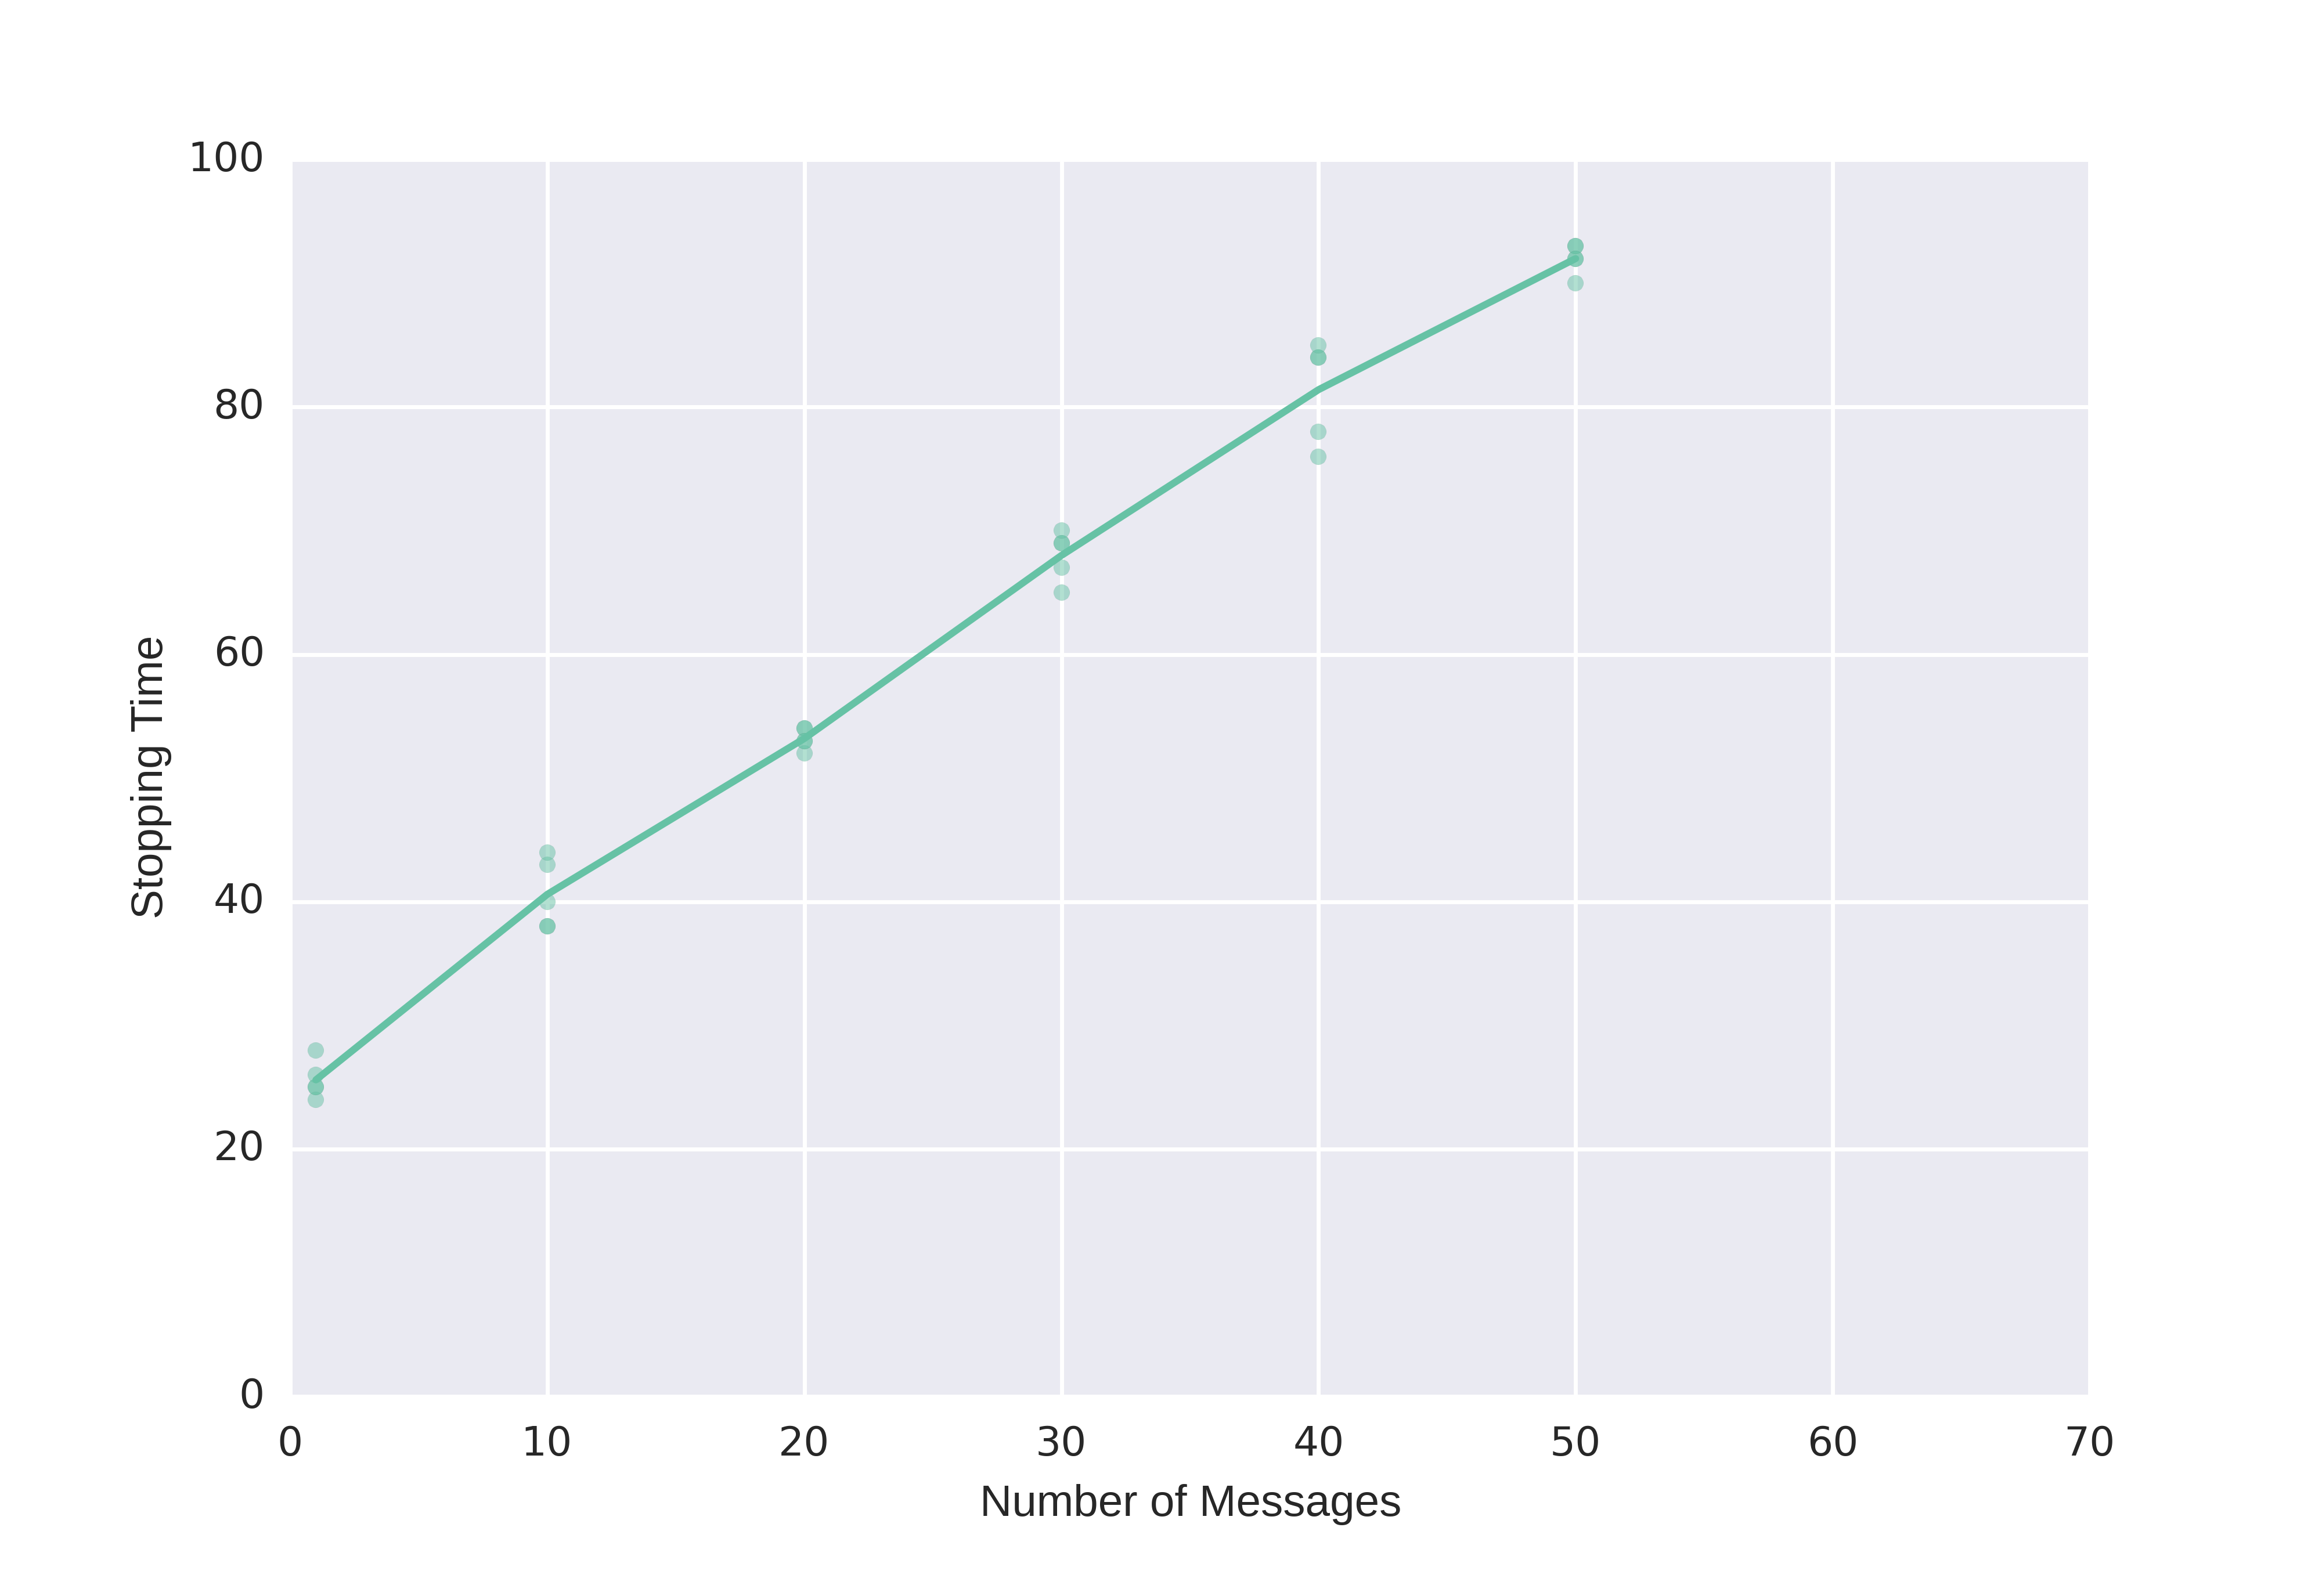
\includegraphics[width=\linewidth]{figures/rlnc-vary-k.png}
\caption{The number of rounds that it takes for the algorithm to terminate is linear in the number in the number of messages}
\label{fig:rlnc-vary-k}
\end{figure} 
\begin{figure}
\centering
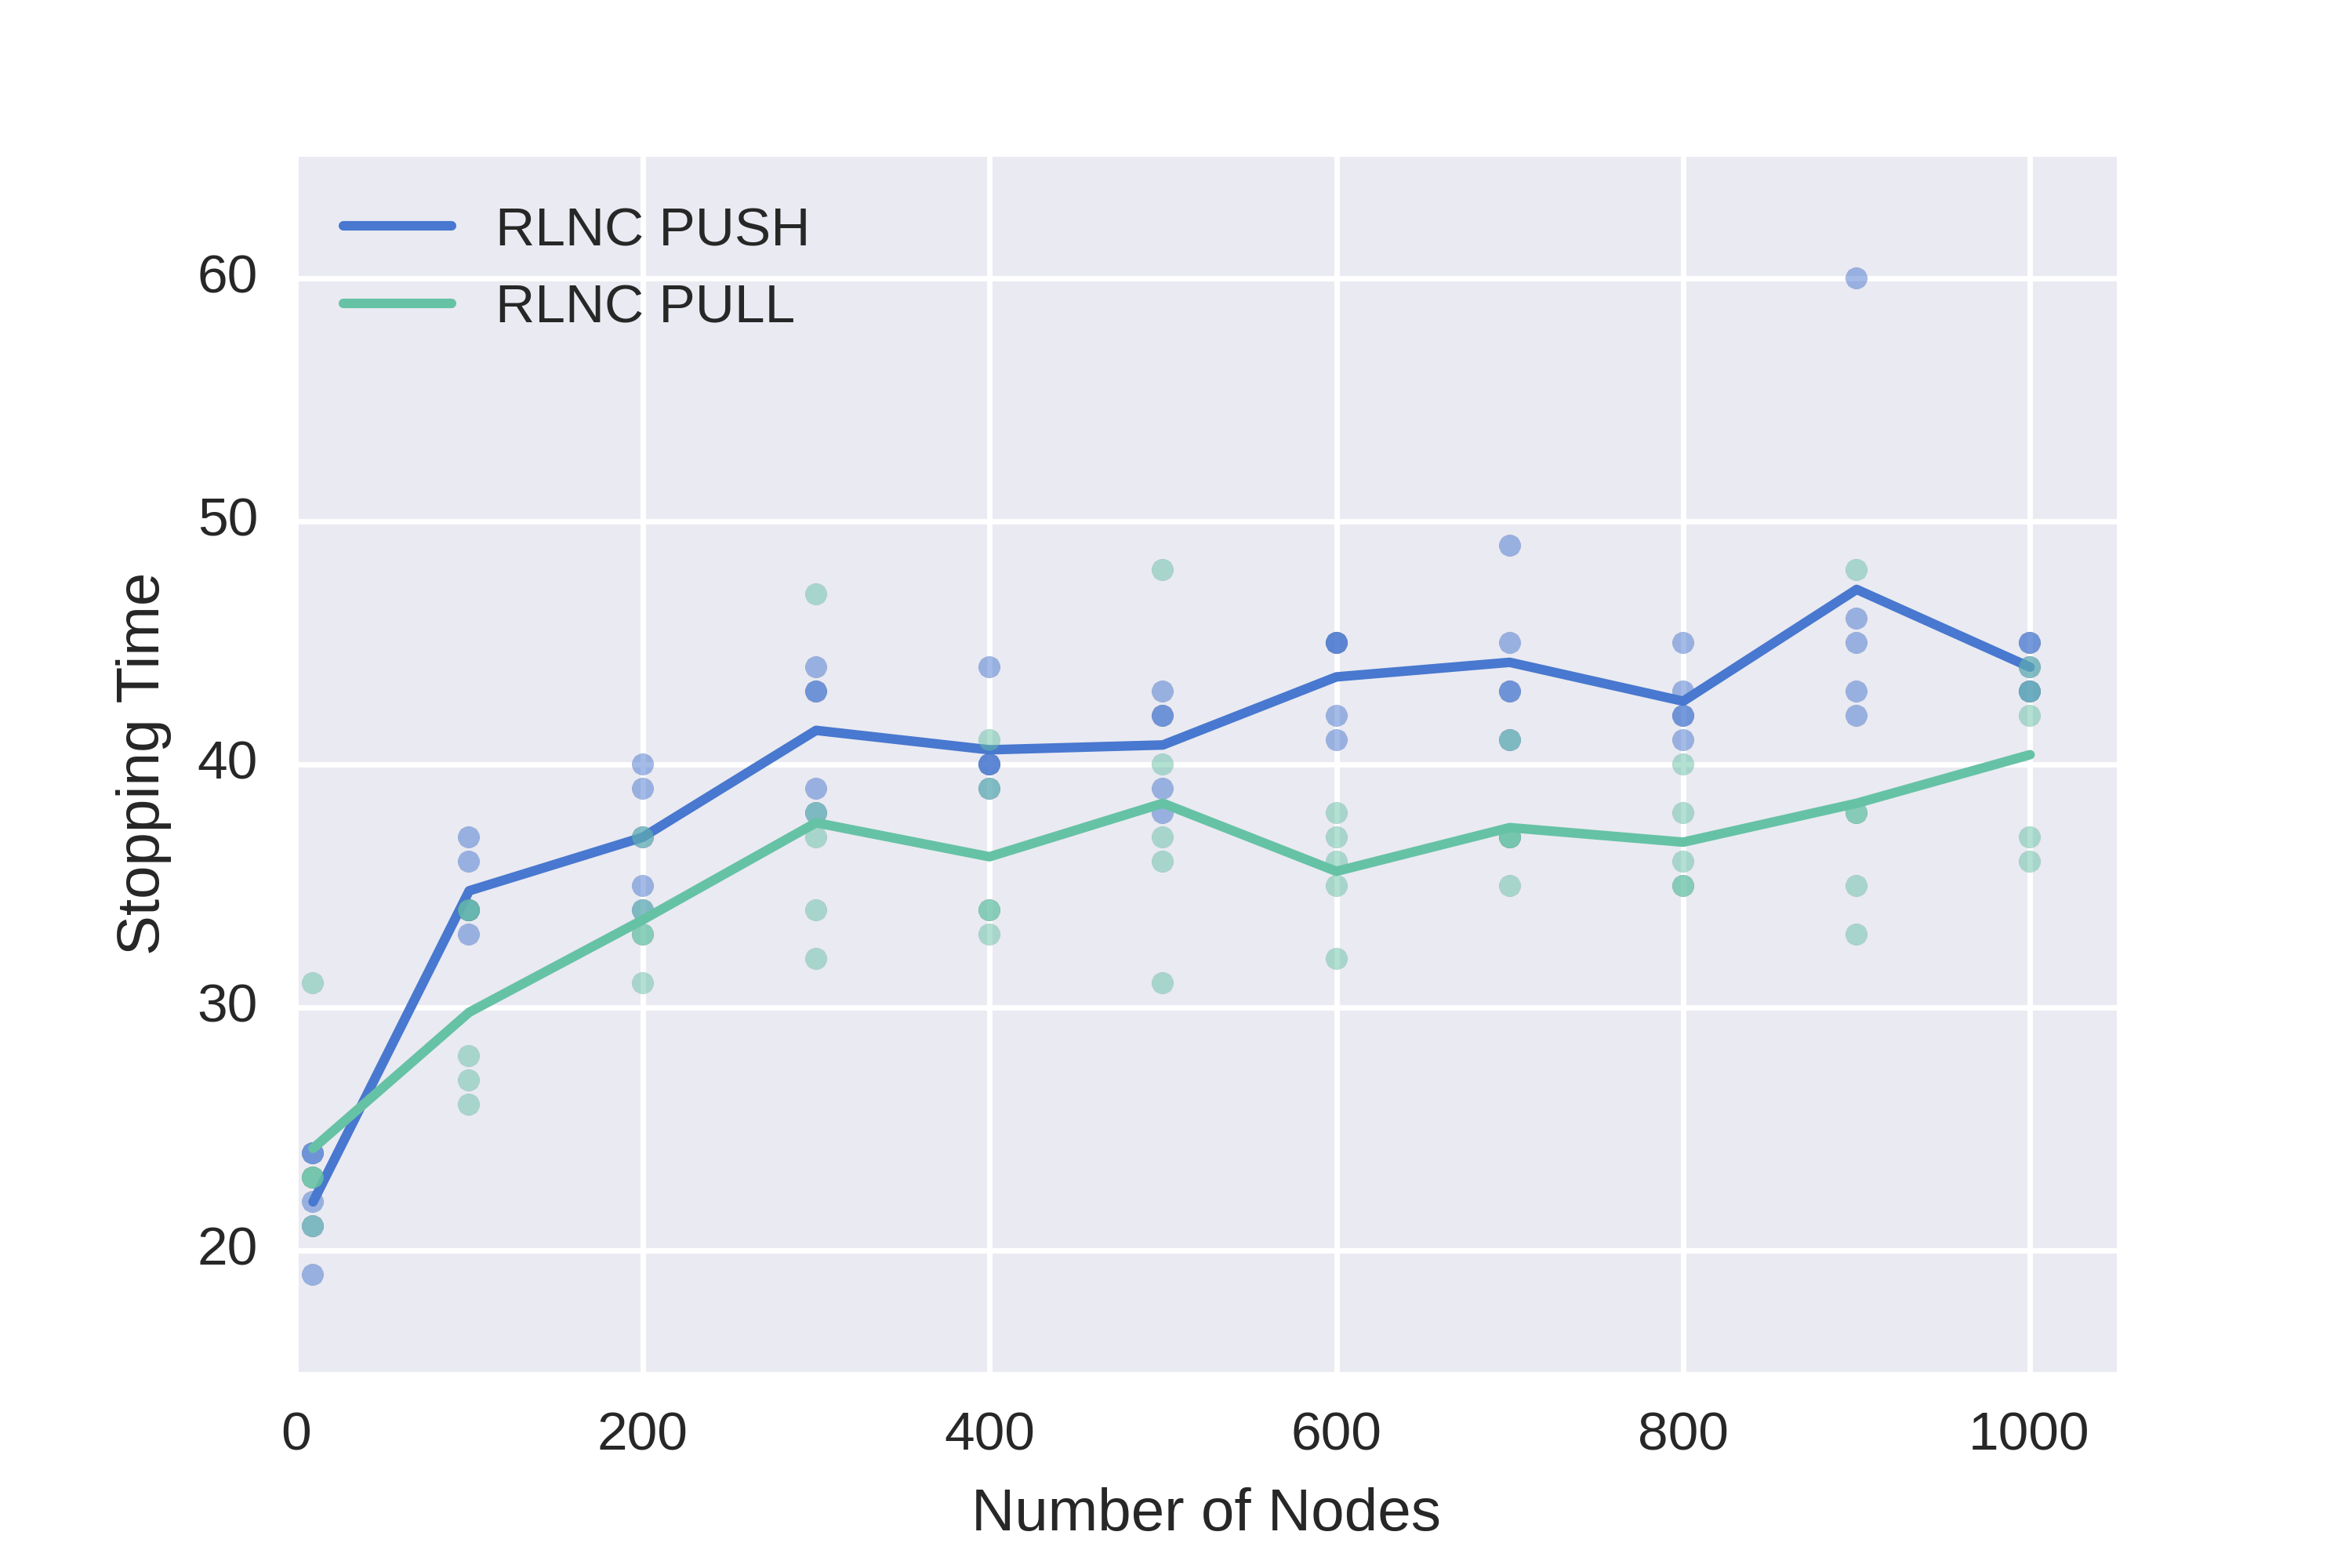
\includegraphics[width=\linewidth]{figures/rlnc-vary-n.png}
\caption{The number of rounds that it takes for the algorithm to terminate is logarithmic in the number of nodes}
\label{fig:rlnc-vary-n}
\end{figure} 


\subsection{Discussion}

\subsection{Conclusions}

\nocite{*}
\bibliographystyle{ieeetr}
\bibliography{nips}



%For my project, I plan to read \emph{Analyzing network coding gossip made easy} and \emph{Epidemic algorithms for replicated database maintenance}. I plan to implement the gossip algorithm with RLNC and perform experiments to measure the stopping time. I will investigate the performance on static graphs vs dynamic graphs, on different starting knowledge configurations, and I will investigate the impact of the different ways in which nodes can connect with each other: broadcasting, pushing, pulling, and exchanging. I will compare my results with the theoretical stopping times given in \cite{haeupler2011analyzing}.



\end{document}